All projects in this dissertation are based on two types of information, register data and genotype data. The registers are used to define the study population, acquire phenotype information for individuals, and link family members. The genotype data is used to run a genome-wide association study (See \cref{sec:GWAS} for details). 

\subsection{Danish Registers}
The Danish registers provide the main source of phenotypic information and allow us to link individuals to their family members. The registers can be linked to one another through a unique 10-digit number assigned to every Dane and resident in Denmark since 1968. In \cref{fig:registerBubbles} is a brief overview of which registers are used and how they are linked. Details on the mentioned registers will be provided in this section.


\subsubsection{The Civil Registration System}
The Danish Civil Registration System was established on the $ 2^{nd} $ of April $ 1968 $, and all persons living in Denmark were registered for administrative use. All registered individuals were given a 10-digit unique personal identification number, commonly referred to as the CPR-number. The CPR-number is used to link individuals across all registers. This register holds information on gender, date of birth, place of birth, citizenship, identity of parents, and is continually updated with information on vital status, place of residence and spouses. On the $ 1^{st} $ of May $ 1972  $ all persons living in Greenland were also included into this register\cite{pedersen2011danish}. 

\subsubsection{The National Patient Register}
The Danish National Patient Register was established in 1977. It has been expanded several times since it was created. Originally, it contained only information on patients admitted to somatic wards. In 1995, the register was expanded to also include outpatients, patients from emergency rooms, and patients from psychiatric wards. In 1994, the international classification of disease, version 10 (ICD-10) was adopted in Denmark, and prior to the adoption, ICD-8 was used\cite{lynge2011danish}. 


\subsubsection{The Psychiatric Central Research Register}
\begin{wrapfigure}{R}{7cm}
	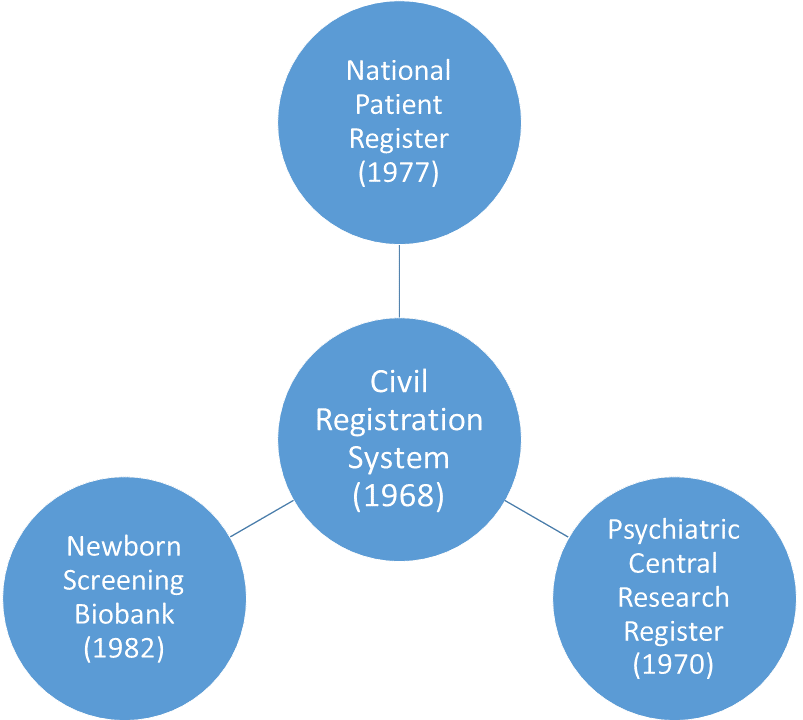
\includegraphics[width=7cm]{intro/registers.png}
	\oldcaption{\sl Illustration of a selected number of Danish registers. They are linked together by the civil registration system. The year denotes the year the register starts.}
	\label{fig:registerBubbles}
\end{wrapfigure}

The psychiatric Central Research Register has valid data from 1970 and onwards. At the beginning, the register contained information on every admission to a mental hospital and psychiatric department, where information such as dates of onset, end of treatment, and all diagnosis were recorded. In 1995, the register became an integrated part of the Danish national patient register and was expanded to also record information from psychiatric emergency room and outpatient treatment. Similar to the national patient register, ICD-10 codes were used after 1995, and ICD-8 were used before. Note that most mild and moderate affected individuals are treated by general practitioners or in private practices, in which case they are not recorded in this register.\cite{mors2011danish}


\subsubsection{The Newborn Screening Biobank}
The Danish Newborn Screening Biobank contains dried blood spot samples from nearly every newborn since 1982. The samples are taken from a heel prick a few days after birth and are stored at $ -20 $\textcelsius. Each year about $ 65,000 $ new samples are added, resulting in over $ 1.8 $ million samples in $ 2007 $. The purpose of the biobank is, among other things, to screen for various diseases at birth. The samples are kept for research purposes, and the dried blood spots provide the basis for the iPSYCH cohort\cite{norgaard2007storage}.

\subsection{Cumulative Incidence Proportions} \label{sec:CIPs}
Another important aspect of the Danish registers is their usage in estimating population representative incidence proportions stratified by sex and year of birth. These CIPs are essential for estimating the thresholds used by LT-FH++, as they are used to account for age-of-onset. All CIPs used throughout our work were estimated by the aid of the Aalen-Johansen estimator with death and emigration as competing events\cite{hansen2017estimating}. 
The Aalen-Johansen estimator of the survival function was used instead of the Kaplan-Meier estimator, as it accounts for competing events, i.e. different causes of censoring (death vs. independent censoring). As the Kaplan-Meier estimator estimates the overall survival function, it always overestimates the risk and can only approximate the true cumulative incidences in the presence of competing risks\cite{andersen2012competing}. As the CIPs are stratified by sex and birth year, they can be interpreted as the proportion of individuals born in a specific year and of a given sex that are diagnosed with an underlying disorder prior to time point $ t $. The data from the registers described above provide the basis for estimating these CIPs and an example of depression CIPs is provided in \cref{fig:CIP_DEP}. They are estimated for each birth year available in the Danish registers, but only shown for every fifth year. The red colour represents women's CIP and the blue is the men's CIP.


\subsection{Genotype Data}
This section covers the sources of genotype data used in this dissertation. There are two main sources, namely iPSYCH and UKBB. Here, we provide a brief overview for both of them. Notably, the iPSYCH cohort is a Danish biobank and has been linked to the previously mentioned registers, as shown in \cref{fig:registerBubbles}. 


\subsubsection{iPSYCH}
\begin{wrapfigure}{O}{8cm}
	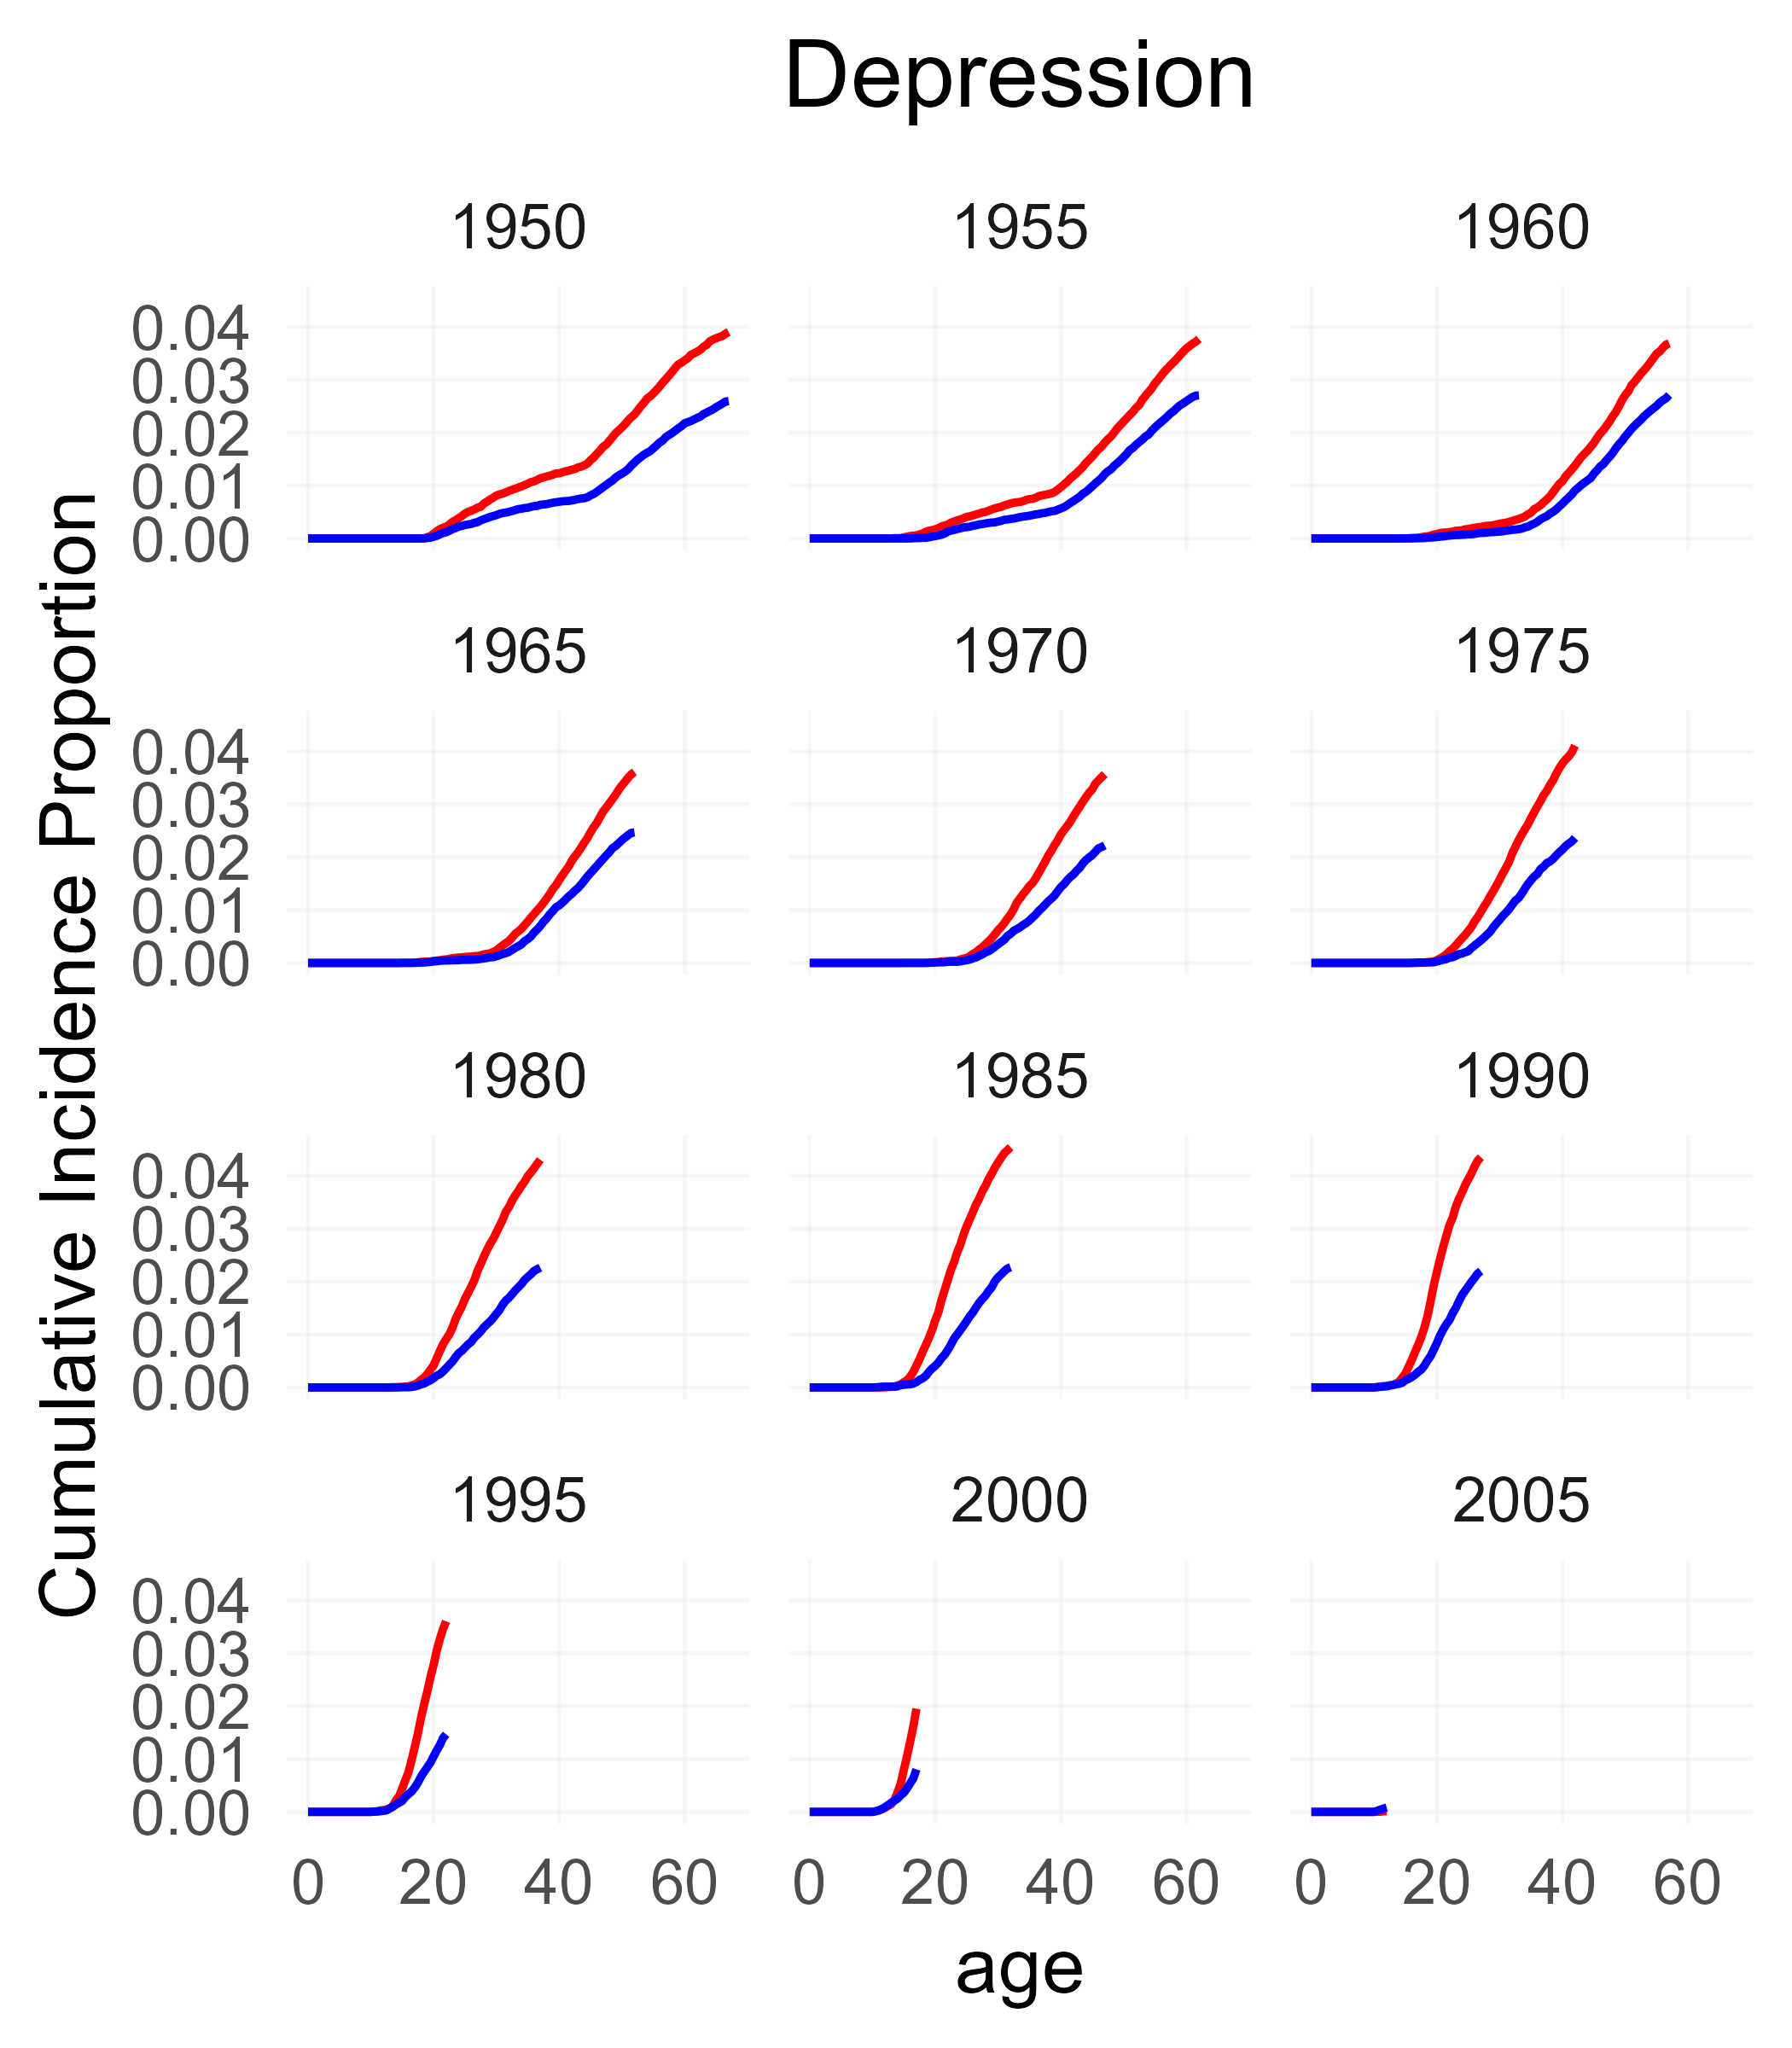
\includegraphics[width=8cm]{methods/prevalencePlot_DEP.png}
	\caption[Cumulative incidence proportions from the Danish 
	Registers]{
		\sl Depression cumulative incidence proportions estimated from the 
		Danish registers. The CIPs have been stratified by birth year and sex. The 
		red colour represent women and the blue represent men. The CIPs are 
		calculated for each birth year, but are only shown in steps of $ 
		5 $ years.}
	\label{fig:CIP_DEP}
\end{wrapfigure}
iPSYCH is a key source of genotype data used in this dissertation. The benefit of a biobank such as iPSYCH is not the number of genotypes, instead its strength is due to the richness of the register information that it is linked to. All of the previously mentioned Danish registers have been linked to the genotypes, allowing for a very detailed set of phenotypes, as well as multiple information on each individual and their family members. The iPSYCH cohort focuses on psychiatric disorders, namely Attention Deficit Hyperactivity Disorder (ADHD), Autism Spectrum Disorder, Anorexia Nervosa, Bipolar disorder, Depression, and Schizophrenia\cite{pedersen2018ipsych2012}. Ethical approval was given by the Danish Scientific Ethics Committee, the Danish Health Data Authority, the Danish data protection agency, and the Danish Neonatal Screening Biobank Steering Committee.

The iPSYCH cohort has been sampled in two rounds. The first round is called iPSYCH2012 and has $ 86,189 $ samples, while the second round, iPSYCH2015i, has $ 56,233 $ samples. The combined cohort is called iPSYCH2015 and has $ 141,265 $ unique samples. The population that iPSYCH2012 is nested within is defined as all singletons born in Denmark between the $ 1^{st} $ of May $ 1981 $ and the $ 31^{st} $ of December $ 2005 $, where the mother is known and the child is alive and living in Denmark by their first birthday. iPSYCH2015i extended the study population to individuals born between $ 1^{st} $ of May $ 1981 $ and $ 31^{st} $ of December $ 2008 $ with the same conditions. In total, $ 1,657,449 $ individuals satisfy this condition. For the first round of sampling, $ 30,000 $ samples were chosen at random, creating a population representative control group. For iPSYCH2015i another $ 21,000 $ were sampled for the control group. From the study population, all individuals with at least one of the focus disorders were sampled for iPSYCH2015 resulting in $ 93,608 $ samples, and $ 50,615 $ population controls. However, due to the random sampling $ 385 $ were chosen as controls for both iPSYCH2012 and iPSYCH2015i and another $ 2,958 $ individuals had at least one of the disorders iPSYCH focuses on, and would have been sampled either way\cite{pedersen2018ipsych2012,bybjerg2020ipsych2015}.

\subsubsection{UK Biobank}

UK Biobank is the second main provider of the genotype data used in our studies. Since $ 2006 $, UKBB has evolved into one of the largest and most detailed, long-term biobank studies in the world, and its impact on the field of statistical genetics should not be underrated. As opposed to the Danish registers and iPSYCH, UKBB's main advantage is its accessibility. It has open access, and it is possible for researchers from all over the world to gain access to the database by simply providing a summary of the research that is intended to be conducted, a description of any new data or variables that will be generated, and information on the UK Biobank data-fields that are required \cite{bycroft2018uk,biobank2015genotyping}. 

As already mentioned, the UK Biobank is one of the largest of its kind, as it includes about $ 500,000 $ individuals. In addition, it has a large amount of environmental, lifestyle, and genetic data that is extended regularly. Among the information provided by the UKBB is genomic data of more than $ 800,000 $ genome-wide variants, electronic health-related records, and web-based questionnaires. 

Since $ 2011 $, there has been questionnaires on diet, cognitive function, occupational history, mental health, digestive health, chronic pain, food preferences, mental well-being as well as health and well-being. Regarding genetic data, it is possible to access genotypes and imputed variants therefrom for $ 488,000 $ participants, whole-exome sequences for $ 470,000 $ participants and whole genome sequences for $ 200,000 $ participants (with more to follow)\cite{van2020exome,bycroft2018uk,ukbbdatatypes}. With respect to the electronic health-related records, primary care data is available for approximately $ 230,000 $ participants, hospital inpatient data is available for all participants. Death and cancer data is available due to the linkage to national death and cancer registries. 

The phenotypic information linked to all UK Biobank participants is quite detailed. UKBB receives cancer registry data from the Information Centre and Information Service Division on a quarterly basis, and the records holds information on the data of cancer diagnosis, the participant's age at cancer diagnosis, the ICD-10 and ICD-9 codes for the type of cancer, the reported occurrences of cancer, the histology code as well as the behaviour code \cite{ukbbcancerlinkage}. 

In addition, UKBB receives death registry data from NHS Digital and the NHS Central Register every six month at the latest. The death records are similar to the cancer registry data and hold information on the date of death, the ICD-10 code for the primary cause of death, the ICD-10 code for the secondary cause of death, as well as the origin and format of the death record. Up until $ 2019 $, some of the death records also contain free-text cause of death information from the death certificate describing the sequence leading to death\cite{ukbbdeathlinkage}.

However, one prevailing disadvantage of the UK Biobank is the lack of registered family history. The available data regarding family members was obtained through touchscreen questionnaires and include only information on parents and siblings that the participants were able (or willing) to share. More precisely, the data contains information about the illnesses of the adopted or biological father, mother, and siblings, as well as the number of adopted or full brothers and sisters. Even more restrictive is the number of diseases that have been considered in these questionnaires, which is only 12. Participants were asked whether their adopted or biological parents and siblings had been diagnosed with severe depression, Parkinson's disease, Alzheimer's disease (dementia), diabetes, high blood pressure, chronic bronchitis (emphysema), breast, bowel, prostate or lung cancer, stroke, or heart disease. This number is low compared to the total number of registered phenotypes, which is several thousands. 

Even if family history is not commonly used in statistical genetics at the present time, it has been included in analyses performed within epidemiology and other fields for many years\cite{schendel2022evaluating,johns2001systematic,guttmacher2004family,runeson2003family}. Recently, some methods accounting for family history, such as GWAX and LT-FH, have been proposed, highlighting the necessity to include high quality health records for family members in biobanks. 

